\clearpage
\section{Additional reference implementations on the ensemble test subsets}
\label{app:matchedbaselines}
The baseline tables answer whether the library offers better predictions than
the additional reference implementations on the cases used by the ensembles.
We score each baseline on the same evaluation rows within each of the three
partitions, excluding that partition's fitting cases. Training uses a
single seed, and provenance determines which saved predictions are eligible.
The verified comparison contains 273 baseline entries across 21 PDE datasets.
For fidelity basis FNO on Heat II and Burgers, we regenerate errors from the
fixed final campaign checkpoints on identified test inputs, replacing archived
scores whose case correspondence was unverified. These entries are included
without retraining. ERA5 is the climate dataset
and uses its separate input disjoint experiment. Its twelve completed baseline
entries and training mean control are scored on exactly the same seven evaluation
inputs as all nine library members and their ensembles. These twelve entries
represent eleven independent fits, because B10 reuses B9. ERA5 has complete
baseline coverage for B1 to B11. The additional controls B12 and B13 are outside
the ranked comparison, and a dash marks an unavailable control.

Baselines follow the training settings of the evaluated benchmark implementations,
with adaptations documented in Appendix~\ref{app:adaptations}.
Source file hashes, saved target identities, or checkpoint evaluation establish case correspondence.
Where field storage has lower precision, a global normalization scale and
storage rounding are allowed when checking row identity. Reported errors use
the original numerical predictions. These checks establish common evaluation
cases, while training budgets, validation procedures, and inference precision
remain different across implementations. They therefore support comparison
under a common test set, without establishing equal training cost or total
fine label exposure. Repeated partitions share trained models and do not
estimate training seed variance.

For example, the inspected Darcy recipes allocate 360 fine rows to fitting and
40 to internal validation for B3 to B5, whereas B1, B2, and the library transfer
recipe fit 400 rows before ensemble fitting. The former still consume 400
fine labels, but their fitting and validation roles differ. Additional
fitting examples are counted separately. These comparisons describe the
available recipes rather than attributing the error differences to architecture
or multifidelity information alone. Some saved timing fields measure prediction
export rather than original training, so they cannot support a common training
cost estimate. The fitted weights also combine a heterogeneous library that
includes a fine only model. Without a matched fine only ensemble and label
allocation controls, the resulting gain is evidence for combination of this
library, not an isolated multifidelity benefit.

\begin{table}[h!]
\centering\footnotesize\setlength{\tabcolsep}{3pt}
\caption{\textbf{Additional reference implementations on identical test subsets.}
Mean relative $L^2$ errors in percent, averaged over three partitions. B1:
Autoregressive POD GP. B2: Nonlinear POD GP. B3: composite MF MLP. B4: composite MF DeepONet.
B5: the latent MF network. B6: nonlinear decoder transfer. B7: MFRNP adapter.
The last two columns repeat the $K=5$ mixtures on exactly these cases.
ERA5 is a separate row. A dash indicates a result not reported on that split. Imported rows use MFRNP data \citep{niu2024}
and ERA5 reanalysis \citep{hersbach2020}.}
\label{tab:baseline_detail1}
\resizebox{\linewidth}{!}{\begin{tabular}{lrrrrrrrrr}
\toprule
Dataset & B1 & B2 & B3 & B4 & B5 & B6 & B7 & \shortstack[r]{Inverse\\error\\mixture} & \shortstack[r]{Fitted\\mixture} \\
\midrule
Darcy & 3.37 & 3.66 & 4.03 & 6.66 & 5.91 & 5.2 & 12.4 & 2.55 & 2.33 \\
Eikonal & 3.49 & 2.99 & 3.12 & 3.35 & 3.38 & 2.65 & 3.62 & 1.76 & 1.76 \\
Helmholtz & 12.3 & 15.2 & 11.5 & 7.84 & 8.12 & 99.6 & 58.6 & 6.89 & 6.55 \\
Poisson I & 0.00731 & 0.00531 & 0.181 & 0.161 & 0.1 & 0.479 & 6.79 & 0.008 & 0.00788 \\
Poisson II$^{\dagger}$ & 0.0128 & 0.0306 & 0.635 & 1.72 & 0.849 & 3.93 & 11.7 & 0.0125 & 0.0129 \\
Pressure Poisson$^{\dagger}$ & 0.457 & 0.472 & 0.07 & 1.53 & 0.127 & 0.446 & 1.05 & 0.0769 & 0.0802 \\
Heat I & 0.326 & 0.327 & 0.0696 & 0.125 & 0.069 & 0.432 & 1.29 & 0.00593 & 0.0062 \\
Heat II & 0.312 & 0.312 & 0.111 & 0.183 & 0.0721 & 0.219 & 7.4 & 0.00437 & 0.00435 \\
Cavity & 0.307 & 0.409 & 23.9 & 4.99 & 0.0419 & 24.1 & 55.7 & 0.142 & 0.142 \\
Navier Stokes & 2.8 & 2.48 & 2.08 & 4.01 & 3.71 & 7.08 & 25.7 & 1.52 & 1.5 \\
Rayleigh Bénard & 0.283 & 0.295 & 0.0542 & 0.0588 & 0.0134 & 0.0613 & 4.5 & 0.00286 & 0.00269 \\
Burgers & 2.16 & 2.5 & 1.54 & 8.14 & 1.22 & 15.7 & 27.7 & 0.513 & 0.502 \\
Euler & 5.6 & 5.54 & 6.56 & 6.16 & 6.15 & 8.81 & 9.15 & 5.64 & 5.73 \\
Porous medium & 1.15 & 0.859 & 0.299 & 1.31 & 0.772 & 0.918 & 33.7 & 0.0262 & 0.0263 \\
Allen Cahn & 55.5 & 98.6 & 59.9 & 44.8 & 41.2 & 94.4 & 69 & 37.9 & 34.6 \\
Cahn Hilliard I$^{\dagger}$ & 29.7 & 27.8 & 53.5 & 48.7 & 27.6 & 61.1 & 74.7 & 11.3 & 10.7 \\
Cahn Hilliard II & 64.8 & 83.5 & 85 & 53.7 & 49.8 & 72.4 & 66.7 & 47.2 & 49.3 \\
Fisher KPP & 6.86 & 6.86 & 6.48 & 4.01 & 3.45 & 7.44 & 4.08 & 2.53 & 2.3 \\
Phase field crystal & 83.5 & 86.4 & 90.7 & 87.5 & 87.8 & 152 & 89.4 & 83.8 & 83.3 \\
Shallow water & 1.14 & 1.02 & 0.467 & 0.878 & 0.691 & 0.883 & 5.59 & 0.357 & 0.389 \\
Wave & 27.7 & 24.9 & 3.3 & 42.3 & 46.6 & 5.39 & 93.9 & 4.39 & 4.27 \\
\midrule ERA5 & 5 & 6.74 & 45 & 16.8 & 5.05 & 23.9 & 19.5 & 5.81 & 6.49 \\
\bottomrule
\end{tabular}
}
\end{table}

\begin{table}[t]
\centering\footnotesize\setlength{\tabcolsep}{3pt}
\caption{\textbf{Remaining reference implementations.}
B8: fidelity basis FNO. B9: FNO transfer I. B10: FNO transfer II.
B11: affine POD GP. B12: parameter kNN. B13: training mean.
B9 and B10 are archived entries for the same inspected recipe, with unresolved
score provenance in the historical PDE archives. For ERA5 and the four additional reaction diffusion datasets, B10 explicitly
reuses B9 predictions with no additional training. Neither comparison treats them as
two distinct baseline families.
Units, partitions, and mixture columns match Table~\ref{tab:baseline_detail1}.
A dash indicates an absent control on the current split.
ERA5's B13 entry is its training mean control.
Imported rows use MFRNP data \citep{niu2024} and ERA5 reanalysis \citep{hersbach2020}.}
\label{tab:baseline_detail2}
\resizebox{\linewidth}{!}{\begin{tabular}{lrrrrrrrr}
\toprule
Dataset & B8 & B9 & B10 & B11 & B12 & B13 & \shortstack[r]{Inverse\\error\\mixture} & \shortstack[r]{Fitted\\mixture} \\
\midrule
Darcy & 5.55 & 5.27 & 5.28 & 3.6 & 21.5 & 38 & 2.55 & 2.33 \\
Eikonal & 2.21 & 2.33 & 2.34 & 4.88 & 5.51 & 31.8 & 1.76 & 1.76 \\
Helmholtz & 99.7 & 4.12 & 4.12 & 15.9 & 25.7 & 92 & 6.89 & 6.55 \\
Poisson I & 0.239 & 0.0804 & 0.0806 & 2.68 & 7.51 & 31.9 & 0.008 & 0.00788 \\
Poisson II$^{\dagger}$ & 82.1 & 0.355 & 0.357 & 2.01 & 12.3 & 38.5 & 0.0125 & 0.0129 \\
Pressure Poisson$^{\dagger}$ & 0.684 & 0.0639 & 0.0645 & 0.681 & 0.196 & 1.58 & 0.0769 & 0.0802 \\
Heat I & 0.275 & 0.0207 & 0.0206 & 1.09 & 1.35 & 12.4 & 0.00593 & 0.0062 \\
Heat II & 0.32 & 0.0202 & 0.0201 & 0.405 & 0.856 & 13.2 & 0.00437 & 0.00435 \\
Cavity & 0.129 & 0.622 & 0.666 & 37.2 & 0.077 & 17.1 & 0.142 & 0.142 \\
Navier Stokes & 1.62 & 1.52 & 1.52 & 21.6 & 3.27 & 41.2 & 1.52 & 1.5 \\
Rayleigh Bénard & 0.78 & 0.0113 & 0.011 & 0.715 & 0.0575 & 9.1 & 0.00286 & 0.00269 \\
Burgers & 0.928 & 0.562 & 0.562 & 11.7 & 0.677 & 73.2 & 0.513 & 0.502 \\
Euler & 7 & 6.52 & 6.43 & 6.25 & 6.21 & 32.2 & 5.64 & 5.73 \\
Porous medium & 5.14 & 0.0718 & 0.0718 & 1.98 & 1.92 & 31.9 & 0.0262 & 0.0263 \\
Allen Cahn & 48.9 & 55.8 & 55.8 & 55.4 & 78.3 & 100 & 37.9 & 34.6 \\
Cahn Hilliard I$^{\dagger}$ & 14.2 & 13.4 & 13.3 & 72.3 & 20.6 & 99.9 & 11.3 & 10.7 \\
Cahn Hilliard II & 54.4 & 54 & 54 & 64.8 & 78 & 100 & 47.2 & 49.3 \\
Fisher KPP & 4.74 & 3.24 & 3.24 & 6.86 & 5.67 & 6.86 & 2.53 & 2.3 \\
Phase field crystal & 102 & 86.8 & 86.8 & 83.5 & 86.7 & 87.5 & 83.8 & 83.3 \\
Shallow water & 0.806 & 0.403 & 0.403 & 2.94 & 1.22 & 25.1 & 0.357 & 0.389 \\
Wave & 25.9 & 6.6 & 6.6 & 50.3 & 42.8 & 98.7 & 4.39 & 4.27 \\
\midrule ERA5 & 5.15 & 11.9 & 11.9 & 8.45 & 5.16 & 6.74 & 5.81 & 6.49 \\
\bottomrule
\end{tabular}
}
\end{table}

\subsection{Elo ranking across all datasets}
\label{app:elo}
Table~\ref{tab:paperbaselines} ranks the nine library members, eleven additional
baseline entries, and three ensemble rules on all 22 datasets, including ERA5.
Each pair of methods plays one comparison per dataset using its unrounded
mean relative $L^2$ error. The lower error wins, and an absolute difference
below $10^{-12}$ is a tie. Cases and fitting partitions are averaged before
these comparisons, so datasets receive equal weight regardless of their
number of evaluation cases. Every method is ranked on the same 22 datasets
in the present reporting collection, with no further exclusions for the Elo calculation.

Following the benchmark ranking procedure, each method starts at 1500.
For methods $a$ and $b$ with ratings $R_a$ and $R_b$, the expected score and
rating update are
\begin{equation}
 p_a=\frac{1}{1+10^{(R_b-R_a)/400}},\qquad
 R_a'=R_a+32(s_a-p_a),\qquad R_b'=R_b-32(s_a-p_a).
\end{equation}
Here $s_a$ is one for a win, zero for a loss, and one half for a tie, and
primed ratings denote the updated values.
The update raises a winner's rating and lowers a loser's rating. A tie moves
the ratings toward each other when they differ.
We reset ratings and shuffle all comparisons independently 500 times, then
report each method's mean final rating. The random order seeds are fixed in
the reporting code. Rows are sorted by unrounded Elo, while displayed ratings
are rounded to integers. This descriptive ranking measures how often a method
wins, rather than the size of its error reduction. It does not estimate
statistical significance or equalize training resources. B9 and B10 remain
separate reported entries of the same transfer recipe, as elsewhere in the paper.

\subsection{Method sources and implementation scope}
The provenance tables connect each evaluated implementation to the component
or modeling idea that motivated it. The results concern these adaptations,
whose differences from the complete published methods are documented in
Appendix~\ref{app:adaptations}. In particular, fidelity basis FNO omits the
continuous fidelity ODE and GP, the latent MF network omits both the variational
last layer and active acquisition, and the all pairs recipe uses fidelity pairs
rather than Poseidon's time pairs.
The latter is inspiration for pair enumeration, not an implementation of the
Poseidon foundation model. FNO transfer builds on multifidelity transfer
\citep{lyu2023}, with FiLM conditioning where indicated \citep{perez2018}.

\begin{table}[t]
\centering\footnotesize\setlength{\tabcolsep}{3pt}
\caption{Sources and adaptations for the nine ensemble members.}
\label{tab:portfolio}\begin{tabular}{p{.045\linewidth}p{.20\linewidth}p{.23\linewidth}p{.39\linewidth}}
\toprule
ID & Implementation & Source & Adaptation and inclusion rationale \\
\midrule
M1 & FiLM FNO transfer & \citep{li2021fno,perez2018,lyu2023} & Coordinate input and parameter FiLM at every FNO block, with LF to HF transfer. Tests repeated conditioning and spectral transfer. \\
M2 & All pairs FNO & \citep{li2021fno,perez2018,herde2024} & Fidelity labels and repeated target supervision. Poseidon is pair enumeration inspiration only. No source field input. \\
M3 & ConvNeXt transfer & \citep{liu2022convnext,ronneberger2015,perez2018,lyu2023} & ConvNeXt blocks in a U shaped field decoder, parameter FiLM, and LF to HF transfer. Tests local spatial processing. \\
M4 & Distribution FNO & \citep{yu2026fire,li2021fno} & FIRE distribution summaries become spatial channels from five LF FNOs. A trained residual FNO replaces foundation model inference. \\
M5 & Wavelet transfer & \citep{tripura2022wno,perez2018,lyu2023} & WNO motivates a custom single level db4 coefficient mixer with FiLM and transfer training. \\
M6 & Retrieved field DeepONet & \citep{lu2021,lu2022mf} & Parameters and a nearest neighbour LF training field enter the branch. The residual needs no new coarse solve. \\
M7 & POD GP & \citep{higdon2008} & HF field SVD and shared coefficient GP hyperparameters. Basis emulation inspiration, not the original Bayesian model. \\
M8 & Slice attention corrector & \citep{wu2024transolver,perez2018} & Changed pooling and cell to slice attention, parameter FiLM, and six corrections of a predicted coarse field. \\
M9 & ConvNeXt corrector & \citep{liu2022convnext,ronneberger2015,perez2018} & ConvNeXt blocks in a U shaped corrector with FiLM. Six updates refine a predicted coarse field rather than generating it directly. \\
\bottomrule
\end{tabular}

\end{table}
\begin{table}[t]
\centering\footnotesize\setlength{\tabcolsep}{3pt}
\caption{Sources and adaptations for the additional reference implementations.}
\begin{tabular}{p{.045\linewidth}p{.20\linewidth}p{.23\linewidth}p{.39\linewidth}}
\toprule
ID & Implementation & Source & Adaptation and inclusion rationale \\
\midrule
B1 & Autoregressive POD GP & \citep{kennedy2000} & KOH inspired scalar field coupling plus a separate residual POD GP. Not joint probabilistic co kriging. \\
B2 & Nonlinear POD GP & \citep{perdikaris2017} & NARGP inspired coefficient kernel with shared covariance hyperparameters and Monte Carlo LF uncertainty. \\
B3 & Composite MF MLP & \citep{meng2020} & Meng inspired pointwise LF network and staged linear plus nonlinear HF corrections. \\
B4 & Composite MF DeepONet & \citep{howard2023} & Howard inspired LF sensor prediction and staged linear plus nonlinear DeepONets. \\
B5 & Latent MF network & \citep{li2022dmfal} & DMFAL inspires two latent levels. Deterministic MSE replaces the probabilistic objective and acquisition. \\
B6 & Nonlinear decoder transfer & \citep{seidman2022} & NOMAD motivates a custom nonlinear coordinate decoder. Multifidelity behavior comes from transfer training. \\
B7 & MFRNP adapter & \citep{niu2024} & Upstream MFRNP model with data, normalization, resize, batching, context, and training adaptations. \\
B8 & Fidelity basis FNO & \citep{li2022ifc} & IFC inspires fidelity dependence. Spatial basis FNO omits the original neural ODE and GP. \\
\bottomrule
\end{tabular}

\end{table}
\begin{table}[t]
\centering\footnotesize\setlength{\tabcolsep}{3pt}
\caption{Transfer variants and classical controls.}
\begin{tabular}{p{.045\linewidth}p{.20\linewidth}p{.23\linewidth}p{.39\linewidth}}
\toprule
ID & Implementation & Source & Adaptation and inclusion rationale \\
\midrule
B9 & FNO transfer I & \citep{lyu2023} & Parameters concatenated with coordinates and LF to HF transfer. Same inspected recipe as B10. \\
B10 & FNO transfer II & \citep{lyu2023} & Separately archived transfer run with the same inspected model and training code as B9. \\
B11 & Affine POD GP & \citep{zhang2018} & One affine slope and intercept across fields applied to an LF POD GP. Conceptual inspiration only. \\
B12 & Parameter kNN & Reference / control & Training field nearest neighbor reference. \\
B13 & Training mean & Reference / control & Input independent fine training mean. \\
\bottomrule
\end{tabular}

\end{table}

\begin{table}[h!]
\centering\small
\caption{\textbf{Different rules for combining the same nine models.} At $K=5$,
each rule is compared with a model selected using the same five fitting
answers. Lower ratios are better. Wins and losses require changes larger than
1\% across the 21 PDE datasets.}
\label{tab:main}\begin{tabular}{lrrrr}
\toprule
Method & Class balanced & Equal dataset & Wins & Losses \\
\midrule
Selected model & 1.000 & 1.000 & 0 & 0 \\
All pairs FNO & 1.333 & 1.502 & 3 & 15 \\
Uniform (all nine) & 5.919 & 4.944 & 2 & 19 \\
Inverse error mixture & 0.888 & 0.935 & 13 & 5 \\
Fitted mixture & 0.884 & 0.923 & 15 & 5 \\
\bottomrule
\end{tabular}

\end{table}

\begin{figure}[t]
\centering
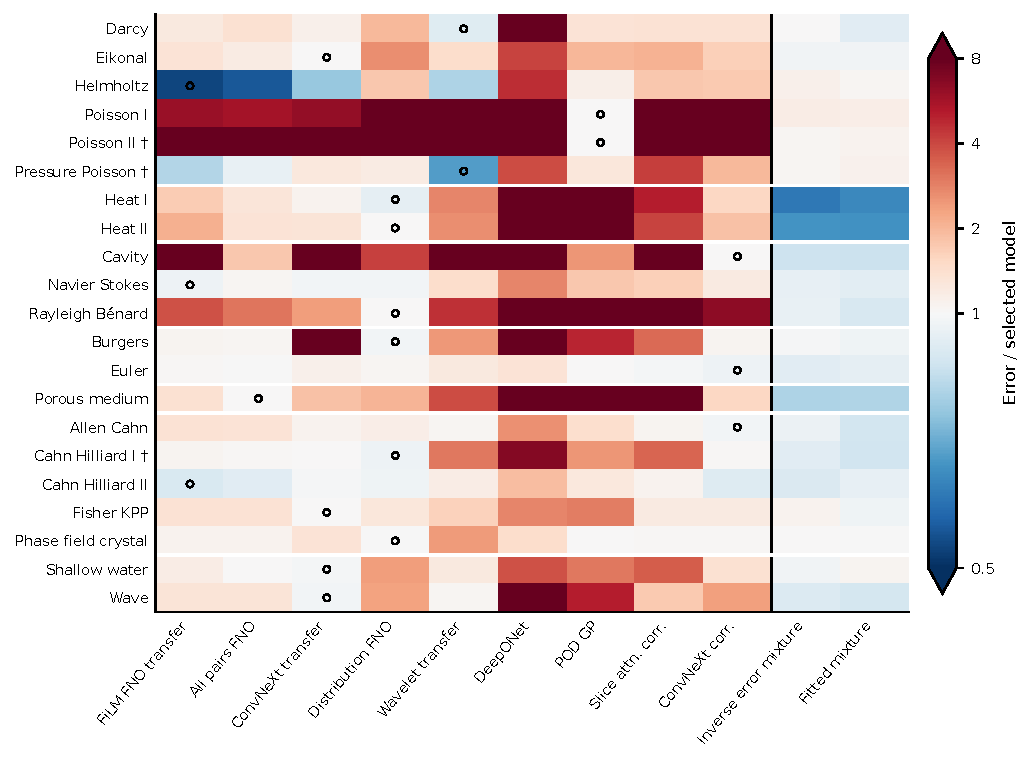
\includegraphics[width=\linewidth]{figures/individual_models.pdf}
\caption{\textbf{Individual models and mixtures on the same evaluation cases.}
Each cell divides a method's mean relative $L^2$ error by the selected model's
error at $K=5$, so blue indicates an improvement. Colors saturate outside
$[0.5,8]$. Circles identify the best individual model after evaluation.
The last two columns fit mixture weights using five additional fine answers,
while the individual models remain fixed. Daggers mark the three audit
exclusions. Appendix~\ref{app:allresults} gives exact errors. Imported datasets
are from \citet{niu2024}.}
\label{fig:individual}
\end{figure}

\subsection{From a trained surrogate library to a deployed ensemble}\label{app:algorithm}
\refstepcounter{algorithm}\label{alg:calibration}
\begin{center}
\fbox{\begin{minipage}{0.94\linewidth}\small
\textbf{Algorithm \thealgorithm: train models, fit the ensemble, and predict}\par
\textbf{Input:} LF/HF training tables, $K$ reserved fine cases, fixed model recipes,
and one prescribed rule: Selected model, Inverse error mixture, or Fitted mixture.\par
1. Check input identities and working grids within the dataset. Train the surrogate models
using training data only. Record unresolved units or simulation metadata.\par
2. Predict fields for the fitting inputs and compute $G_1,\ldots,G_K$.\par
3. Fit the prescribed rule on all $K$ cases using the definitions in Section~\ref{sec:method}.\par
4. Save preprocessing, model identities, and fitted weights.\par
\textbf{Predict:} combine model predictions at new parameters using Equation~\eqref{eq:mixture}.\par
\textbf{Evaluate:} score reserved fine answers only after saving these choices.
\end{minipage}}
\end{center}
The algorithm separates surrogate training from ensemble fitting. The bundled
program implements steps 2 to 4 and combines saved model predictions for new
inputs. Dataset adapters and base model training remain separate components.
The three rules use the same fitting and evaluation cases within each comparison.


\subsection{Field comparison example}
\label{app:fieldcomparison}
Figure~\ref{fig:fieldcomparison} uses Heat I as an illustrative success case
selected after examining the dataset results. Within that dataset, it shows
the first evaluation input of the first partition, rather than the case with
the largest gain. The five fitting inputs are disjoint from this case, and all
weights are reused from the saved fits. The nine prediction archives are
verified by their source hashes and input identities. Recomputing error
products from the plotted fields reproduces the stored error matrix.
Across all 20 evaluation inputs in this partition, the fitted mixture has
lower relative $L^2$ error than every individual model. The main aggregate
comparisons include the other partitions and datasets, including failures.

The top row uses one linear color scale for all predicted and true fields.
The bottom row shows absolute error with one shared logarithmic color scale,
linear between zero and $10^{-5}$ so exact zeros remain visible. Its limits
cover every plotted value. No field values are smoothed or modified, and each
reported relative $L^2$ error is computed on the complete $64\times64$ grid.
The three comparison columns show the selected model, inverse error mixture,
and fitted mixture. The selected model is M4, chosen using the fitting examples,
so its column reproduces M4. The source package includes
the field arrays, extraction manifest, plotting script, and numerical checks.

\clearpage
\section{Visual inventory of every dataset}
\label{app:gallery}
The gallery illustrates the structures that the models must learn.
The first five plates enlarge the 21 PDE fields in Figure~\ref{fig:datasets},
and the sixth enlarges ERA5. Every example is row zero of its HF training table,
selected by a fixed rule independent of prediction errors. Numerical color scales show the
stored target values and coordinate labels denote native array indices. Heat
fields span space and time. The ERA5 illustration uses the native
$721\times1440$ array, while predictions and losses use a $128\times256$ working
grid. Its supplied metadata do not establish the physical units or target
transformation, so the colors cannot be read as absolute temperatures. The
sample arrays and extraction manifest preserve shapes, hashes, source paths,
and this fixed selection rule. Imported fields are from MFRNP \citep{niu2024}
and ERA5 reanalysis \citep{hersbach2020}.

The cavity target is vorticity, not velocity or streamfunction. Its field
values range from about $-391$ to $195$, while 90\% of grid values lie between
$-7.44$ and $2.98$. A linear full range makes the interior appear almost constant.
We use a symmetric logarithmic scale for the cavity panel, linear within
$[-1,1]$, with limits $[-400,400]$. Square geometry is preserved and no values
are clipped or altered. Cavity displays its first training field at
$\mathrm{Re}=594.23$. Array rows increase upward from the bottom wall,
and the top lid moves to the right. This display change does not change any
model inputs, targets, or reported errors.

\begin{figure}[h!]
\centering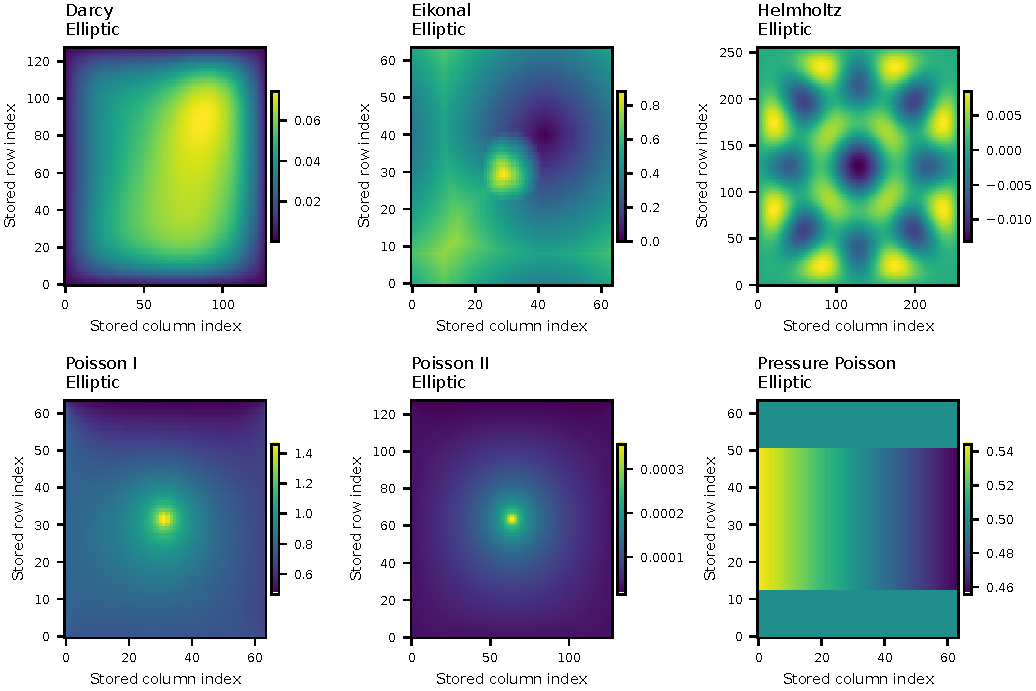
\includegraphics[width=\linewidth]{figures/dataset_detail_1.pdf}
\caption{Elliptic HF training examples, entries 1 to 6 in the main gallery.
Poisson II is from \citet{niu2024}.}
\end{figure}
\begin{figure}[t]
\centering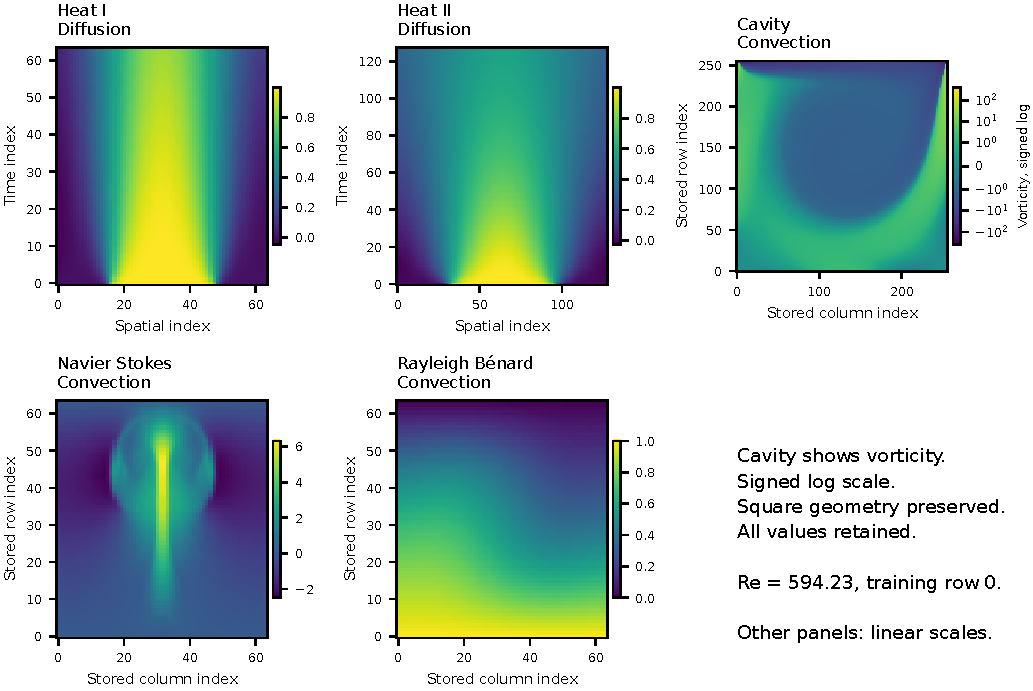
\includegraphics[width=\linewidth]{figures/dataset_detail_2.pdf}
\caption{Diffusion and convection HF training examples, entries 7 to 11 in the
main gallery. Heat II and Navier Stokes are from \citet{niu2024}. The cavity panel
uses a signed logarithmic scale.}
\end{figure}
\begin{figure}[t]
\centering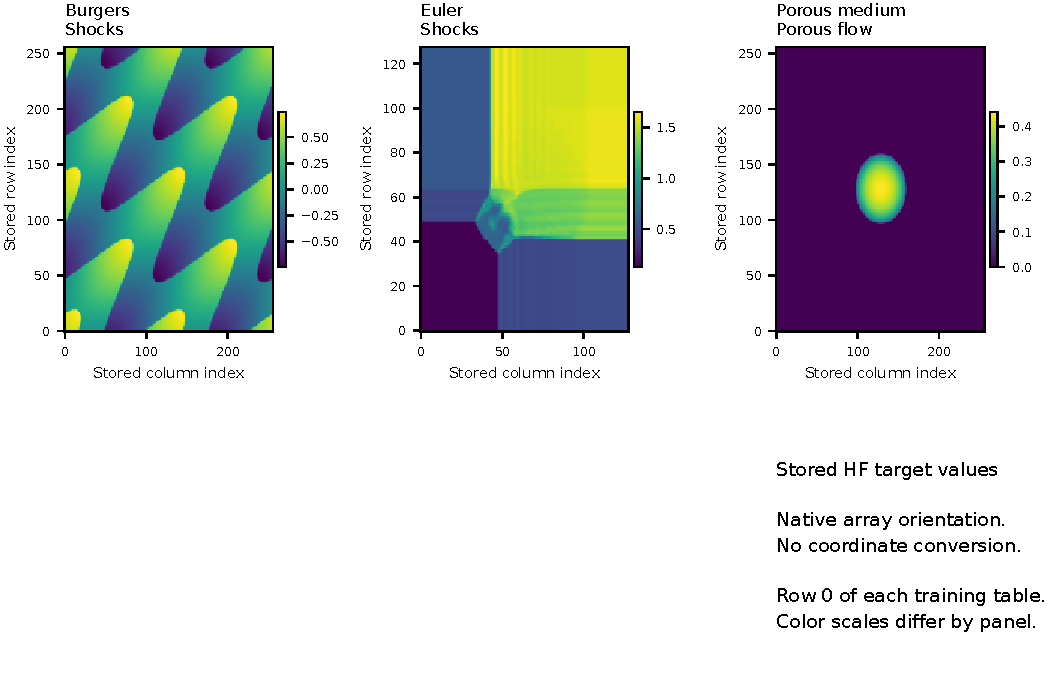
\includegraphics[width=\linewidth]{figures/dataset_detail_3.pdf}
\caption{Shock and porous flow HF training examples, entries 12 to 14 in the main gallery.}
\end{figure}
\begin{figure}[t]
\centering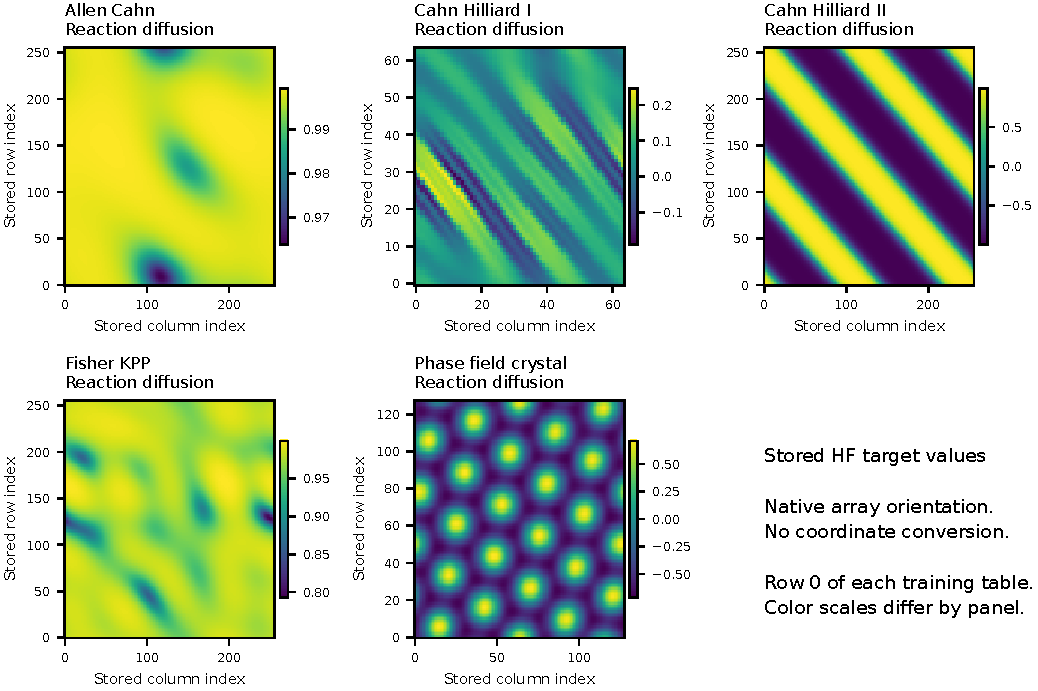
\includegraphics[width=\linewidth]{figures/dataset_detail_4.pdf}
\caption{Reaction diffusion HF training examples, entries 15 to 19 in the main
gallery, with Cahn Hilliard I and II shown together.}
\end{figure}
\begin{figure}[t]
\centering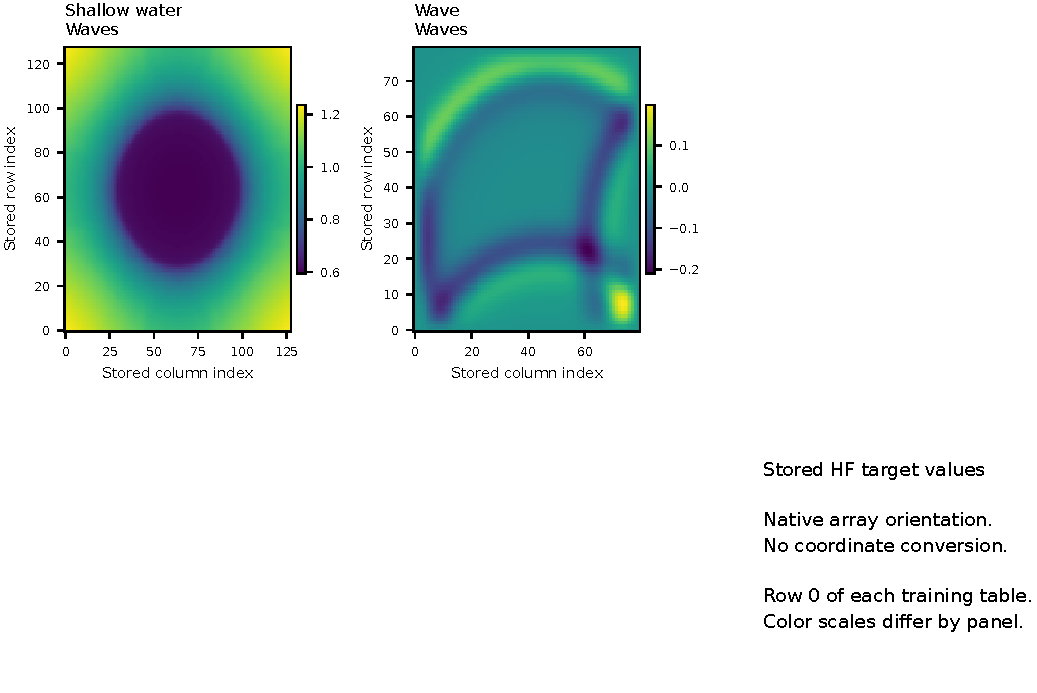
\includegraphics[width=\linewidth]{figures/dataset_detail_5.pdf}
\caption{Wave HF training examples, entries 20 and 21 in the main gallery.}
\end{figure}
\begin{figure}[t]
\centering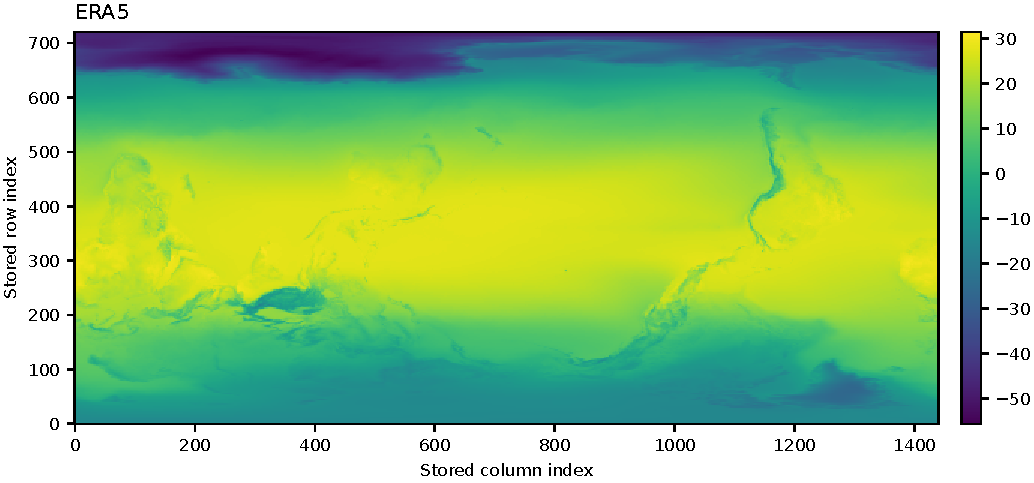
\includegraphics[width=\linewidth]{figures/dataset_detail_6.pdf}
\caption{HF training example for ERA5 \citep{hersbach2020,niu2024}, the twenty second
dataset in the main gallery. This native $721\times1440$ illustration displays
stored target values. Evaluation uses the $128\times256$ working grid.}
\end{figure}
\clearpage
